% このディレクトリで2回実行：pdflatex -interaction=nonstopmode -halt-on-error resume6An26w.tex
\documentclass[a4paper,10pt,pdflatex,ja=standard,jafont=ipaex-type1,
  magstyle=real,scale=1]{bxjsarticle}
\usepackage{lmodern}
\usepackage{amsmath,amssymb,mathtools}
\usepackage{geometry}
\geometry{reset,left=22mm,right=22mm,top=20mm,bottom=17mm,
  headheight=13pt,headsep=6mm,footskip=10mm}
\usepackage{xcolor}
\usepackage{enumitem}
\usepackage{array,booktabs,tabularx}
\usepackage{fancyhdr}
\usepackage{lastpage}
\usepackage{pdfpages}
\usepackage{tikz}
\usetikzlibrary{arrows.meta,calc,decorations.pathreplacing}

\definecolor{ink}{HTML}{193A5C}
\definecolor{accent}{HTML}{237D82}
\definecolor{soft}{HTML}{EAF3F3}
\definecolor{muted}{HTML}{52616B}
\newcommand{\coursename}{解析学 II}
\newcommand{\handoutnumber}{6}
\pagestyle{fancy}
\fancyhf{}
\fancyhead[L]{\small\color{ink}\coursename{}・授業要約と演習}
\fancyhead[R]{\small\color{ink}第\handoutnumber 回}
\fancyfoot[C]{\small\color{ink}\thepage/\pageref{LastPage}}
\renewcommand{\headrulewidth}{0.3pt}
\setlength{\parindent}{0pt}
\setlength{\parskip}{2pt}
\setlength{\abovedisplayskip}{5pt}
\setlength{\belowdisplayskip}{5pt}
\setlength{\abovedisplayshortskip}{3pt}
\setlength{\belowdisplayshortskip}{4pt}
\setlist[itemize]{leftmargin=1.8em,itemsep=1pt,topsep=2pt,parsep=0pt}

\newcommand{\handouttitle}[1]{%
  \begin{center}
    {\Large\color{ink}#1}\par\vspace{3mm}
    {\color{accent}\rule{0.88\linewidth}{0.7pt}}
  \end{center}\vspace{-2mm}}
\newcommand{\handout}[2]{%
  \renewcommand{\handoutnumber}{#1}%
  \handouttitle{第#1回\quad #2}}
\newcommand{\topic}[1]{\par\vspace{5pt}%
  {\large\sffamily\mdseries\color{accent}#1}\par\vspace{2pt}}
\newcommand{\keybox}[1]{\par\vspace{3pt}\begingroup
  \setlength{\fboxsep}{4pt}%
  \colorbox{soft}{\parbox{\dimexpr\linewidth-2\fboxsep\relax}{\small #1}}%
  \endgroup\par\vspace{2pt}}
\newenvironment{problems}
  {\begin{enumerate}[leftmargin=2em,itemsep=3pt,topsep=3pt,parsep=0pt,
    font=\color{accent}]}
  {\end{enumerate}}


\newcommand{\examplelabel}[1]{{\sffamily\mdseries\color{ink}#1}}
\newcommand{\problemspace}{\par\vspace{5mm}}
\newcommand{\exercises}{%
  {\color{accent}\hrule height 0.7pt}\vspace{3pt}%
  \topic{演習問題（6題）}%
  {\small 変換後の式・ヤコビアン・積分範囲を書こう。面積や質量の問題にも同じ公式を使える。}\par}
\tikzset{
  handout diagram/.style={>={Stealth[length=3.2pt,width=3.2pt]},line join=round,
    every node/.style={font=\scriptsize,text=ink}},
  region/.style={fill=soft,draw=accent,semithick},
  slice/.style={accent,line width=1.8pt},
  guide/.style={muted,densely dashed,thin},
  axis/.style={->,ink,thin}}


% 学生コメントと回答を一組にして配置する。
\newcommand{\feedback}[2]{%
  \par\addvspace{3pt}\noindent\begin{minipage}{\linewidth}%
  {\color{ink}Q. #1}\par\vspace{1pt}%
  {\color{accent}A. }#2%
  \end{minipage}\par}
\fancypagestyle{smalltestpages}{%
  \fancyhf{}%
  \fancyhead[L]{\small\color{ink}\coursename{}・小テスト}%
  \fancyhead[R]{\small\color{ink}第5回}%
  \fancyfoot[C]{\small\color{ink}\thepage/\pageref{LastPage}}%
  \renewcommand{\headrulewidth}{0.3pt}}

\begin{document}
\fontsize{10pt}{13.5pt}\selectfont
\setlength{\abovedisplayskip}{4pt}
\setlength{\belowdisplayskip}{4pt}
% 前回の学生コメントと回答を話題ごとにまとめる。
\fancyhead[L]{\small\color{ink}\coursename{}・フィードバック}
\handout{6}{前回のコメントへのフィードバック}
\topic{広義積分と答案の書き方}
\feedback{無限を文字におきかえないと計算できない例を見てみたい}{%
$\displaystyle\int_1^\infty\frac{1}{x(x+1)}\,dx$ などを考えると面白いかもしれないですね。}

\feedback{広義積分で置き換える文字をどうするか}{%
基本好きな文字で良いです。自分は $R$ とかよく使いますが。}

\feedback{中間や期末でも広義積分は極限を取ったほうが良いか？}{%
そうですね、ぜひ取ってください。}

\feedback{本当にこれでいいんだろうかと思ってしまう}{%
小テストの回答を見ている限り、よくできてると思います。記述の仕方も全て正しいと思います。}

\feedback{3）の操作が正当であるかわからないので後で調べたい}{%
正しいですよ。}

\feedback{重心を求める問題に一時間戦ってやっと理解した}{%
その格闘が大事です！}

\topic{中間テストについて}
\feedback{中間テストの難易度}{%
演習やレポートのレベルの問題で作ります。後は皆さんの作る問題次第。}

\feedback{中間テストは同じ形式か？}{%
次回作ってもらった問題を二問くらい出そうと思います。}

\topic{授業と日々のこと}
\feedback{とても寒い、中島もお大事に}{%
ありがとうございます、すっかり風邪をひいてしまいました。}

\feedback{3限が休みでチョーハッピー}{%
よかったですね（にっこり）。}

\feedback{物理と中国語のテストが被っていて大変です}{%
そういう時期なんですね。頑張ってください。}

\feedback{毎回一限これていい感じ}{%
そうですね、早起きできると一日のリズムが整ったような気になります。}

\topic{ちょっとした話題}
\feedback{すきなラーメンは？}{%
二郎系ですね。}

\feedback{無限にとんがっててハッピー}{%
！！？！？！？}

\feedback{ポッキーは？トッポは？}{%
もちろんポッキーです。}

\feedback{今日はポッキーの日だがポッキーが強いからポッキーの日にしたのかポッキーの日と呼ばれるからポッキーが強いのか}{%
やたらポッキーの感想が多いと思ったら今日は11月11日だからポッキーの日なんですね。}
\clearpage

% 前回の小テストの問題と解答を配置する。
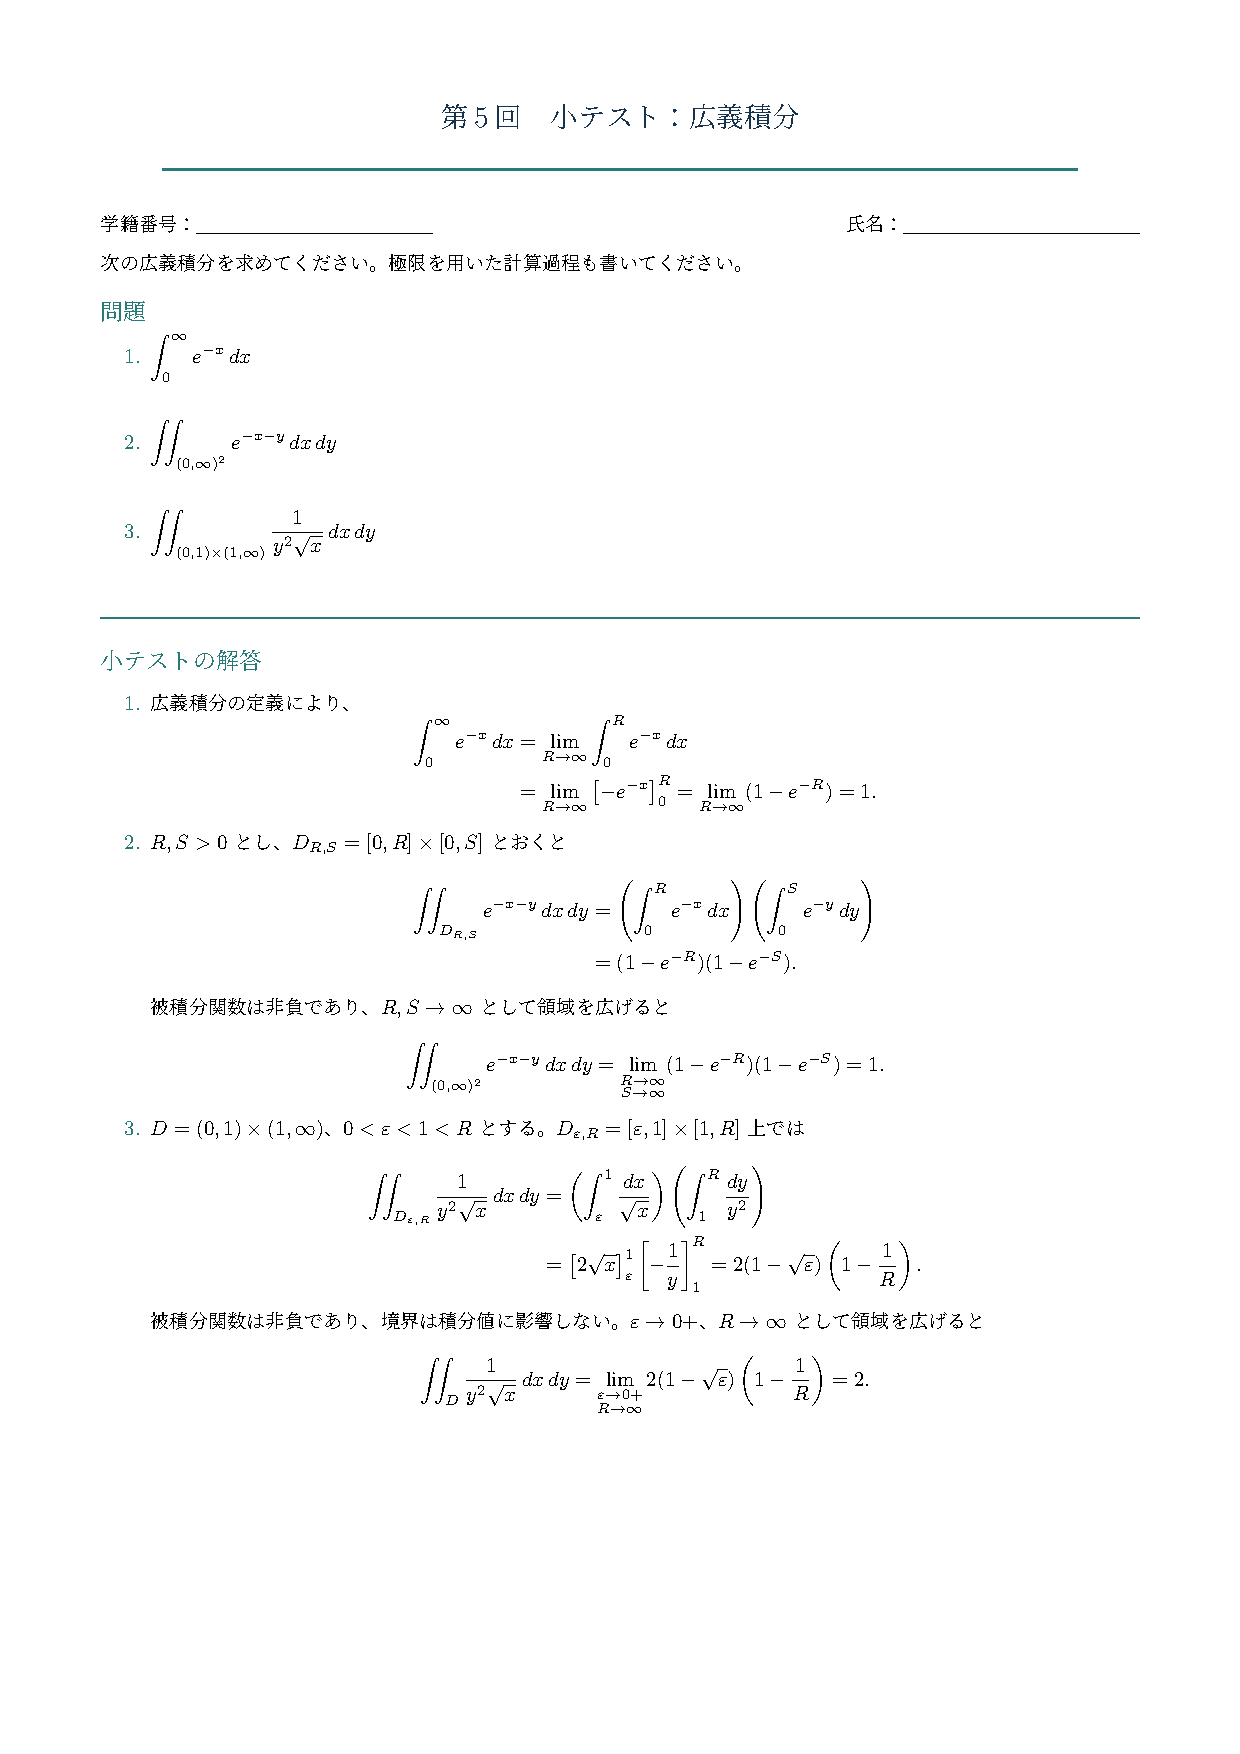
\includepdf[pages=-,pagecommand={\thispagestyle{smalltestpages}}]{smalltest5_review.pdf}
\clearpage

\fancyhead[L]{\small\color{ink}\coursename{}・授業要約と演習}
\fancyhead[R]{\small\color{ink}第\handoutnumber 回}
\handout{6}{重積分の変数変換（ヤコビアン）}\label{lesson-start}
\keybox{到達目標：変換後の領域・関数・面積要素をそろえて重積分を計算できる。
ヤコビアンの絶対値を面積の伸縮率として理解しよう。}

\topic{ヤコビ行列と面積の伸縮率}
座標変換 $T(u,v)=(x(u,v),y(u,v))$ のヤコビ行列と、その行列式を
$$
 DT=\begin{pmatrix}\partial_u x&\partial_v x\\\partial_u y&\partial_v y\end{pmatrix},\qquad
 J_T=\det DT=(\partial_u x)(\partial_v y)-(\partial_v x)(\partial_u y)
$$
とする。$\partial_u x=\partial x/\partial u$ は、$u$ についての偏微分を表す。
微小長方形の2辺は、変換後には $(\partial_u T)\,du$ と $(\partial_v T)\,dv$ で近似される。
その面積は $|J_T|\,du\,dv$ なので
$$
 dx\,dy=|J_T(u,v)|\,du\,dv.
$$
通常の面積では絶対値を取る。$J_T$ の符号は座標の向きの保存・反転を表す。


\par\vspace{2pt}\noindent
\begin{minipage}[b]{0.48\linewidth}\centering
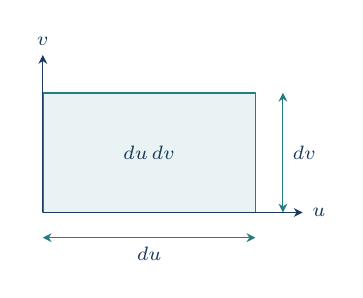
\begin{tikzpicture}[handout diagram,x=1cm,y=0.8cm]
\path[region] (0,0) rectangle (2.7,1.9);
 \draw[axis] (0,0) -- (3.3,0) node[right] {$u$};
 \draw[axis] (0,0) -- (0,2.5) node[above] {$v$};
 \draw[<->,accent] (0,-0.4) -- (2.7,-0.4) node[midway,below] {$du$};
 \draw[<->,accent] (3.05,0) -- (3.05,1.9) node[midway,right] {$dv$};
 \node at (1.35,0.95) {$du\,dv$};
\end{tikzpicture}\par
{\small\color{muted}変換前：小さな長方形}\par
\end{minipage}\hfill
\begin{minipage}[b]{0.48\linewidth}\centering
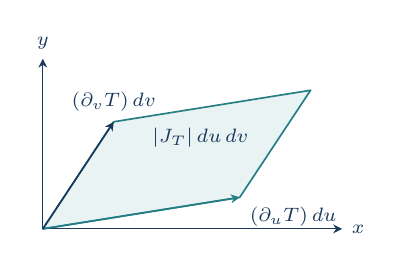
\begin{tikzpicture}[handout diagram,x=1cm,y=0.8cm]
\path[region] (0,0) -- (2.5,0.5) -- (3.4,2.2) -- (0.9,1.7) -- cycle;
 \draw[axis] (0,0) -- (3.8,0) node[right] {$x$};
 \draw[axis] (0,0) -- (0,2.7) node[above] {$y$};
 \draw[->,accent,semithick] (0,0) -- (2.5,0.5) node[below right] {$(\partial_u T)\,du$};
 \draw[->,ink,semithick] (0,0) -- (0.9,1.7) node[above] {$(\partial_v T)\,dv$};
 \node at (2,1.45) {$|J_T|\,du\,dv$};
\end{tikzpicture}\par
{\small\color{muted}変換後：接ベクトルが張る平行四辺形}\par
\end{minipage}
\par\vspace{2pt}

\topic{変数変換公式と計算の要点}
元の積分領域を $D$、$(u,v)$ 平面でそれに対応する領域を $E$ とすると
$$
 \iint_Df(x,y)\,dx\,dy
 =\iint_E f(x(u,v),y(u,v))\,|J_T(u,v)|\,du\,dv.
$$
関数・面積要素・積分範囲の3つを同時に書き換える。
同じ点を重複して数えないように、変換に使う範囲を選ぶことに注意。


\topic{線形変換の例}
$x=2u+v$、$y=u+3v$ なら $J_T=\det\begin{pmatrix}2&1\\1&3\end{pmatrix}=5$。
$E=[0,1]^2$ の像 $D$ は平行四辺形で
$$
 \operatorname{Area}(D)=\iint_E5\,du\,dv=5,\qquad
 \iint_D(x+y)\,dx\,dy
 =5\int_0^1\int_0^1(3u+4v)\,dv\,du=\frac{35}{2}.
$$


\par\vspace{2pt}\noindent
\begin{minipage}[b]{0.48\linewidth}\centering
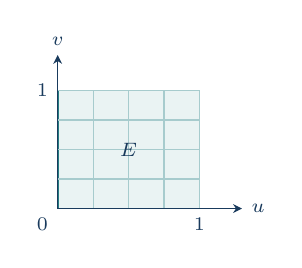
\begin{tikzpicture}[handout diagram,x=0.9cm,y=0.75cm]
\path[region] (0,0) rectangle (2,2);
 \draw[accent!40,step=0.5] (0,0) grid (2,2);
 \draw[axis] (0,0) -- (2.6,0) node[right] {$u$};
 \draw[axis] (0,0) -- (0,2.6) node[above] {$v$};
 \node[below left] at (0,0) {$0$};
 \node[below] at (2,0) {$1$};
 \node[left] at (0,2) {$1$};
 \node at (1,1) {$E$};
\end{tikzpicture}\par
{\small\color{muted}単位正方形の面積は1}\par
\end{minipage}\hfill
\begin{minipage}[b]{0.48\linewidth}\centering
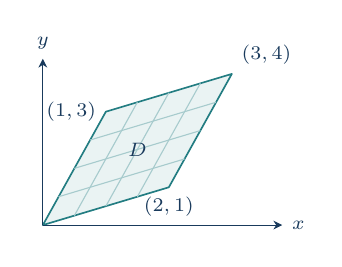
\begin{tikzpicture}[handout diagram,x=0.8cm,y=0.48cm]
\path[region] (0,0) -- (2,1) -- (3,4) -- (1,3) -- cycle;
 \foreach \t in {0.25,0.5,0.75}{
  \draw[accent!40] (2*\t,\t) -- ({2*\t+1},{\t+3});
  \draw[accent!40] (\t,3*\t) -- ({\t+2},{3*\t+1});}
 \draw[axis] (0,0) -- (3.8,0) node[right] {$x$};
 \draw[axis] (0,0) -- (0,4.4) node[above] {$y$};
 \node[below] at (2,1) {$(2,1)$};
 \node[above right] at (3,4) {$(3,4)$};
 \node[left] at (1,3) {$(1,3)$};
 \node at (1.5,2) {$D$};
\end{tikzpicture}\par
{\small\color{muted}$T(u,v)=(2u+v,u+3v)$ で面積は5倍}\par
\end{minipage}
\par\vspace{2pt}

\newpage
% 授業要約の2ページ目の上半分に残りの説明を置く。
\noindent\begin{minipage}[b][\dimexpr0.5\textheight-\parskip\relax][t]{\linewidth}
\topic{極座標：円・扇形・円環に適する座標}
$x=r\cos\theta$、$y=r\sin\theta$、$r\ge0$ とすると
$$
 \det\frac{\partial(x,y)}{\partial(r,\theta)}
 =\begin{vmatrix}\cos\theta&-r\sin\theta\\\sin\theta&r\cos\theta\end{vmatrix}=r,
 \qquad dx\,dy=r\,dr\,d\theta.
$$
半径方向の幅 $dr$ と円弧方向の長さ $r\,d\theta$ の積が面積要素になる。
\par\examplelabel{例：半径 $R>0$ の円板 $D_R$。}
$$
 \iint_{D_R}(x^2+y^2)\,dx\,dy
 =\int_0^{2\pi}\int_0^Rr^3\,dr\,d\theta=\frac{\pi R^4}{2}.
$$


\topic{楕円への変換と板の質量}
$a,b>0$、$x=ar\cos\theta$、$y=br\sin\theta$ なら $|J_T|=ab r$。
楕円 $x^2/a^2+y^2/b^2\le1$ は $0\le r\le1,\ 0\le\theta<2\pi$ に対応する。
\par
面密度が $\rho(x,y)$ の板の質量は $M=\iint_D\rho(x,y)\,dx\,dy$ で求める。
面密度が一定なら、質量は「面密度 $\times$ 面積」となる。
\keybox{ヤコビアンは逆変換のものと取り違えない。極座標では半径の範囲と角度の範囲を図で確認する。}

\par\vspace{2pt}\noindent
\begin{minipage}[b]{0.48\linewidth}\centering
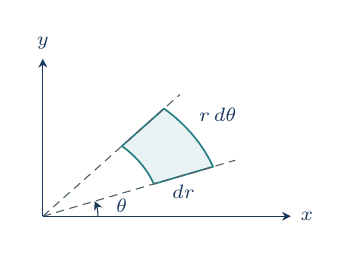
\begin{tikzpicture}[handout diagram,x=1cm,y=0.8cm]
\path[region] (20:1.5) -- (20:2.3) arc[start angle=20,end angle=48,radius=2.3]
   -- (48:1.5) arc[start angle=48,end angle=20,radius=1.5] -- cycle;
 \draw[guide] (0,0) -- (20:2.6);
 \draw[guide] (0,0) -- (48:2.6);
 \draw[axis] (0,0) -- (3.15,0) node[right] {$x$};
 \draw[axis] (0,0) -- (0,2.5) node[above] {$y$};
 \draw[->,ink] (0.7,0) arc[start angle=0,end angle=20,radius=0.7];
 \node at (1,0.16) {$\theta$};
 \node[below] at (20:1.9) {$dr$};
 \node[above right] at (36:2.3) {$r\,d\theta$};
\end{tikzpicture}\par
{\small\color{muted}細い扇形：$dA\approx dr\,(r\,d\theta)$}\par
\end{minipage}\hfill
\begin{minipage}[b]{0.48\linewidth}\centering
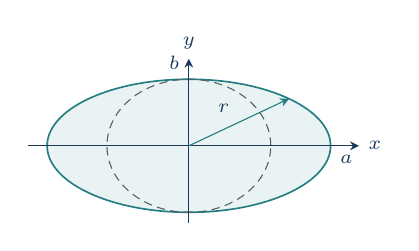
\begin{tikzpicture}[handout diagram,x=0.8cm,y=0.65cm]
\path[region] (0,0) ellipse (2.25 and 1.3);
 \draw[guide] (0,0) circle (1.3);
 \draw[axis] (-2.55,0) -- (2.7,0) node[right] {$x$};
 \draw[axis] (0,-1.5) -- (0,1.7) node[above] {$y$};
 \draw[->,accent] (0,0) -- (1.59,0.92) node[midway,above left] {$r$};
 \node[below right] at (2.25,0) {$a$};
 \node[above left] at (0,1.3) {$b$};
\end{tikzpicture}\par
{\small\color{muted}単位円板を $x$ 方向に $a$ 倍、$y$ 方向に $b$ 倍}\par
\end{minipage}
\par\vspace{2pt}

\end{minipage}\par\nointerlineskip
% 授業要約の2ページ目の下半分に演習問題と書き込み用の余白を置く。
\noindent\begin{minipage}[b][0.5\textheight][t]{\linewidth}
\exercises
\begin{problems}
\item $x=2u$、$y=3v$ の $J_T$ と、単位正方形 $0\le u,v\le1$ を変換した長方形の面積を求めよ。
\problemspace

\item $D=\{(x,y):0\le x+y\le2,\ 0\le x-y\le1\}$ とする。
変数変換で $\iint_D(x+y)e^{x-y}\,dx\,dy$ を求めよ。
\problemspace

\item 台形の板 $D=\{(x,y):1\le x\le2,\ x\le y\le2x\}$ の面密度を $\rho(x,y)=1+(y/x)^2$ とする。
$u=x$、$v=y/x$ とおき、変換後の積分範囲と面積要素を示して、質量 $M=\iint_D\rho(x,y)\,dx\,dy$ を求めよ。
\problemspace

\item 上半円板 $D=\{(x,y):x^2+y^2\le4,\ y\ge0\}$ の面積を、極座標で計算せよ。
\problemspace

\item 内半径 $1$、外半径 $2$ のワッシャーを、円環 $D=\{(x,y):1\le x^2+y^2\le4\}$ として表す。
極座標を用いて面積 $A=\iint_D1\,dx\,dy$ を求めよ。$r$ と $\theta$ の積分範囲も書け。
\problemspace

\item 楕円板 $x^2/4+y^2\le1$ の面積を、$x=2r\cos\theta$、$y=r\sin\theta$ を使って求めよ。
\problemspace

\end{problems}
\end{minipage}

\newpage
\handouttitle{第6回\quad 演習問題の解答}
{\small ヤコビアン・積分範囲・計算結果を、問題文と照らし合わせて確認しよう。}\par
\begin{problems}
\setlength{\itemsep}{9pt}
\item $x=2u$、$y=3v$ より
$$
 DT=\begin{pmatrix}2&0\\0&3\end{pmatrix},\qquad J_T=6.
$$
変換前の範囲は $0\le u,v\le1$ なので、長方形の面積は
$$A=\int_0^1\int_0^1 6\,dv\,du=6.$$

\item $u=x+y$、$v=x-y$ とおくと、$x=(u+v)/2$、$y=(u-v)/2$ より
$$
 J_T=\begin{vmatrix}1/2&1/2\\1/2&-1/2\end{vmatrix}=-\frac12,\qquad
 dx\,dy=\frac12\,du\,dv.
$$
積分範囲は $0\le u\le2$、$0\le v\le1$、被積分関数は $(x+y)e^{x-y}=ue^v$ なので
$$
 \iint_D(x+y)e^{x-y}\,dx\,dy
 =\frac12\int_0^2\int_0^1 ue^v\,dv\,du
 =\frac12\left[\frac{u^2}{2}\right]_0^2[e^v]_0^1=e-1.
$$

\item $u=x$、$v=y/x$ を逆に解くと $x=u$、$y=uv$。
$1\le x\le2$ は $1\le u\le2$ に、$x\le y\le2x$ は $1\le v\le2$ に変わる。
また
$$
 J_T=\begin{vmatrix}1&0\\v&u\end{vmatrix}=u,\qquad
 dx\,dy=u\,du\,dv,\qquad \rho(u,uv)=1+v^2.
$$
したがって、質量は
$$
 M=\int_1^2\int_1^2 u(1+v^2)\,dv\,du
  =\left[\frac{u^2}{2}\right]_1^2
   \left[v+\frac{v^3}{3}\right]_1^2
  =\frac32\cdot\frac{10}3=5.
$$

\item 上半円板の範囲は $0\le r\le2$、$0\le\theta\le\pi$。
面積要素 $dx\,dy=r\,dr\,d\theta$ を用いると
$$
 A=\int_0^{\pi}\int_0^2 r\,dr\,d\theta
  =\pi\left[\frac{r^2}{2}\right]_0^2=2\pi.
$$

\item $x^2+y^2=r^2$ より、ワッシャーの範囲 $1\le x^2+y^2\le4$ は
$1\le r\le2$、$0\le\theta<2\pi$ に対応する。したがって
$$
 A=\iint_D1\,dx\,dy
  =\int_0^{2\pi}\int_1^2 r\,dr\,d\theta
  =2\pi\left[\frac{r^2}{2}\right]_1^2=3\pi.
$$
外側の円板の面積 $4\pi$ から、穴の面積 $\pi$ を引いても同じ値になる。

\item $x=2r\cos\theta$、$y=r\sin\theta$ では $x^2/4+y^2=r^2$ なので、
範囲は $0\le r\le1$、$0\le\theta<2\pi$ となる。また
$$
 J_T=\begin{vmatrix}2\cos\theta&-2r\sin\theta\\\sin\theta&r\cos\theta\end{vmatrix}=2r.
$$
よって、楕円板の面積は
$$
 A=\int_0^{2\pi}\int_0^1 2r\,dr\,d\theta=2\pi.
$$
\end{problems}
\keybox{積分する関数を置き換えたら、面積要素の $|J_T|$ と、変換後の積分範囲も確認しよう。}
\end{document}
